\documentclass[12pt,a4paper]{article}
\usepackage[utf8x]{inputenc}
\usepackage[english,hebrew]{babel}
\usepackage{graphicx}
\usepackage{verbatim}
\usepackage{url}
\usepackage{bm}
\usepackage{float}

\graphicspath{{images/}}

\usepackage{tikz}
\usetikzlibrary{positioning,through,calc,intersections,arrows.meta}
\usepackage{tkz-euclide}
\usetkzobj{all}

%\usetikzlibrary{external}
%\tikzexternalize[prefix=tikz/]

% Use stealth arrows
\tikzset {
  >=stealth
}

\textwidth=15.5cm
\textheight=23cm
\topmargin=0pt
\headheight=0pt
\oddsidemargin=2em
\headsep=0pt
\parindent=0pt
\renewcommand{\baselinestretch}{1.1}
\setlength{\parskip}{0.3\baselineskip plus 1pt minus 1pt}

\newcommand{\bover}[1]{\bm{\overline{#1}}}

\begin{document}
\thispagestyle{empty}

\selectlanguage{hebrew}

%\begin{comment}

\begin{center}
\textbf{\Huge גיאומטריה}

\bigskip
\bigskip
\bigskip

\textbf{\Large מוטי בן-ארי}

\bigskip

\textbf{\Large מכון ויצמן למדע}

\bigskip

\url{http://www.weizmann.ac.il/sci-tea/benari/}

\bigskip

\end{center}

\selectlanguage{english}

\vfill

\begin{center}
\sffamily\copyright{}\  2018 by Moti Ben-Ari.
\end{center}

\begin{footnotesize}
\sffamily
This work is licensed under the Creative Commons Attribution-ShareAlike 3.0 Unported License. To view a copy of this license, visit \url{http://creativecommons.org/licenses/by-sa/3.0/} or send a letter to Creative Commons, 444 Castro Street, Suite 900, Mountain View, California, 94041, USA.
\end{footnotesize}

\begin{center}

\includegraphics[width=.2\textwidth]{../../by-sa.png}
\end{center}

\newpage
\selectlanguage{hebrew}


במסמך זה אביא פתרונות לשאלות על גיאומטריה )שאלה 4( בבחינות הבגרות )שאלון
$806$(.
אנסה לתאר את דרכי החשיבה המובילות לפתרונות עם דגש על בחירת המשפטים שמשתמשים בהם בפתרונות, תוך ציון מספרי המשפטים כפי שמופיע ברשימה של משרד החינוך. בסוף אביא מספר המלצות המבוססות על תהליכי הפתרון.

%\end{comment}

%%%%%%%%%%%%%%%%%%%%%%%%%%%%%%%%%%%%%%%%%%%%%%%%%%%%%%%%%%%%%%%%%%%

\section*{קיץ תשע"ה מועד ב}

\begin{center}
\selectlanguage{english}
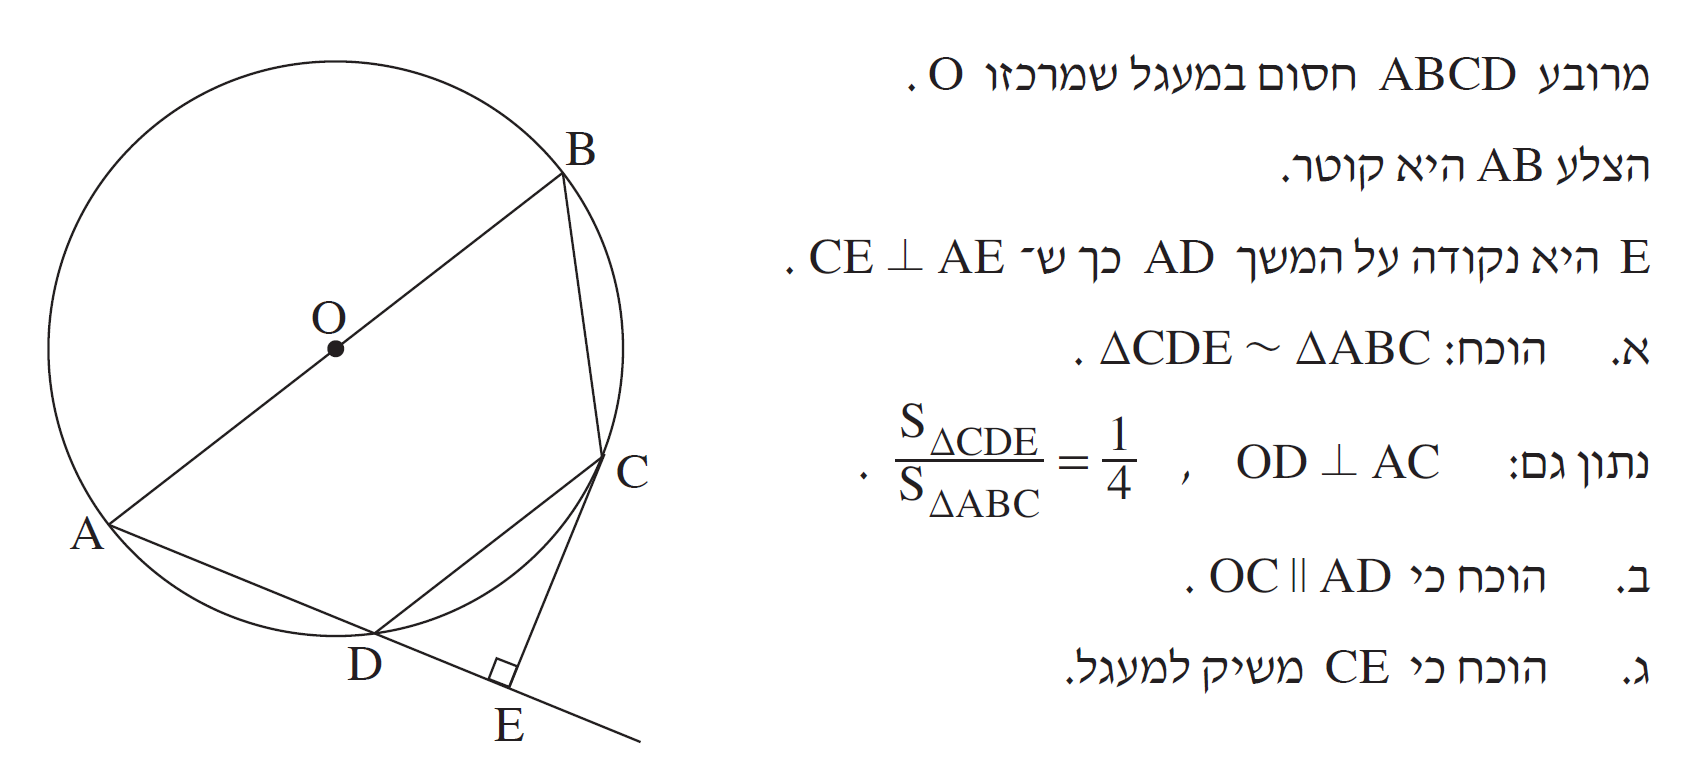
\includegraphics[width=\textwidth]{summer-2015b-4}
\end{center}

\textbf{סעיף א}
$\angle ACB=90^\circ$
כי הוא נשען על קוטר. 
לפי משפט
$(56)$
ניתן לחסום מרובע במעגל רק אם סכום הזוויות הנגדיות שווה ל-%
$180^\circ$,
ולכן
$\angle ADC+\angle ABC=180^\circ$,
אבל
\[
\angle CDE=180-(180-\alpha)=\alpha=\angle ABC\,,
\]
בגלל זוויות משלימות. 
$\triangle ABC \sim \triangle CDE$
לפי ז.ז. )משפט
$98$(.


\begin{center}
\selectlanguage{english}
\begin{tikzpicture}%[scale=1]
\coordinate [label=above:$O$] (O) at (0,0);
\coordinate [label=below left:$A$] (A) at (-2,-2);
\fill (O) circle(1.5pt);
\fill (A) circle(1.5pt);
\node [draw,thick,circle through=(A),name path=circ] (circle) at (O) {};
\path [name path=diam] (A) -- +(45:6);
\path [name intersections={of=circ and diam,by={B}}];
\fill (B) node[above right] {$B$} node[below,xshift=-3pt,yshift=-6pt] {$\alpha$} circle(1.5pt);
\draw[thick] (A) -- (B);
\draw [thick,name path=ad] (A) -- +(-15:5);
\path [name intersections={of=circ and ad,by={dummy1,D}}];
\fill (D) node[below] {$D$} node[right,xshift=10pt,yshift=1pt] {$\alpha$} node[above,xshift=-8pt,yshift=8pt] {$180\!-\!\alpha$} circle(1.5pt);
\path [thick,name path=dc] (D) -- +(45:4);
\path [name intersections={of=circ and dc,by={dummy2,C}}];
\fill (C) node[right] {$C$} circle(1.5pt);
\draw [thick] (D) -- (C) -- (B);
\coordinate (E) at ($(A)!(C)!(D)$);
\fill (E)  node[below] {$E$} circle(1.5pt);
\draw[thick] (C) -- (E);
\draw[rotate=76] (E) rectangle +(5pt,5pt);
\draw[thick,dashed] (A) -- (C);
\draw[rotate=108] (C) rectangle +(5pt,5pt);
\end{tikzpicture}
\end{center}

\textbf{סעיף ב}
היחס בין הצלעות של משולשים דומים שווה לשורש שורש יחס השטחים הנתון )משפט
$100$(.
נחפש צלעות שהיחס ביניהם הוא 
$\frac{1}{2}$.
היתר
$AB=2r$
כך שהצלע המתאים לה במשולש הדומה
$CD$
יהיה באורך
$r$.

המשולש
$\triangle OCD$
שווה שוקיים )אפילו שווה צלעות(, ולכן לפי משפט
$6$
הגובה הנתון
$CF$
הוא גם תיכון. לפי משפט 
$20$\footnote{%
בספרי גיאומטריה משתמשים במשפט זה כדי להוכיח שמשלושים ישר זווית עם צלעות ויתרים שווים חופפים.}
המשולשים
$\triangle OCF,\triangle OAF,\triangle DCF$
חופפים, ו-%
$\triangle ACF$
חופף ל-%
$\triangle OAF$
לפי צ.ז.צ. מכאן ש-%
$OC\|AD$
לפי זוויות מתחלפות
$\angle OCA,\angle CAD$.

\begin{center}
\selectlanguage{english}
\begin{tikzpicture}%[scale=1]
\coordinate [label=above:$O$] (O) at (0,0);
\coordinate [label=below left:$A$] (A) at (-2,-2);
\fill (O) circle(1.5pt);
\fill (A) circle(1.5pt);
\node [draw,thick,circle through=(A),name path=circ] (circle) at (O) {};
\path [name path=diam] (A) -- +(45:6);
\path [name intersections={of=circ and diam,by={B}}];
\fill (B) node[above right] {$B$} node[below,xshift=-3pt,yshift=-6pt] {$\alpha$} circle(1.5pt);
\draw[thick] (A) -- (B);
\draw [thick,name path=ad] (A) -- +(-15:5);
\path [name intersections={of=circ and ad,by={dummy1,D}}];
\fill (D) node[below] {$D$} node[right,xshift=10pt,yshift=1pt] {$\alpha$} circle(1.5pt);
\path [thick,name path=dc] (D) -- +(45:4);
\path [name intersections={of=circ and dc,by={dummy2,C}}];
\fill (C) node[right] {$C$} circle(1.5pt);
\draw [thick] (D) -- node[above] {$r$} (C) -- (B);
\coordinate (E) at ($(A)!(C)!(D)$);
\fill (E)  node[below] {$E$} circle(1.5pt);
\draw[thick] (C) -- (E);
\draw[rotate=76] (E) rectangle +(5pt,5pt);
\draw[thick,dashed,name path=ac] (A) -- (C);
\draw[rotate=107] (C) rectangle +(5pt,5pt);
\draw[thick,dashed,name path=od] (D) -- node[left,near end,yshift=-2pt] {$r/2$} node[left,near start,yshift=-2pt] {$r/2$} (O) -- node[above] {$r$} (C);
\path [name intersections={of=ac and od,by={F}}];
\fill (F) node[above right] {$F$} circle(1.5pt);
\draw[rotate=107] (F) rectangle +(5pt,5pt);
\path (A) -- node[above] {$r$} (O) -- node[above] {$r$} (B);
\end{tikzpicture}
\end{center}
בפתרונות אחרים שראיתי, משתמשים בעובדה ש-%
$\triangle OCD$
הוא שווה צלעות ולכן הזוויות שלו הן
$60^\circ$.
לא מצאתי שערך זה נחוץ כדי להוכיח את הטענה.

\textbf{סעיף ג}
כדי להוכיח ש-%
$CF$
משיק למעגל, נשמתמש במשפט )
$78$(
ונוכיח שהזווית 
$\angle ECO$
בינו לבין הרדיוס
$CO$
היא זווית ישרה. כאן כן נשתמש בעובדה ש-%
$\triangle OCD$
הוא שווה צלעות ולכן הזווית
$\angle OCD$
הוא
$60^\circ$.
בסעיף א הוכחנו ש-%
$ABC\sim CDE$
כך ש-%
$\angle CAB = \angle ECD$.
בסעיף ב הוכחנו ש-%
$AC$
הוא חוצה זווית של
$\angle OAD$.
מכאן ש-%
\[
\angle ECO = \angle ECD + \angle OCD = 30^\circ + 60^\circ = 90^\circ\,.
\]

%\begin{comment}

%%%%%%%%%%%%%%%%%%%%%%%%%%%%%%%%%%%%%%%%%%%%%%%%%%%%%%%%%%%%%%%%%%%

\section*{קיץ תשע"ה מועד א}

\begin{center}
\selectlanguage{english}
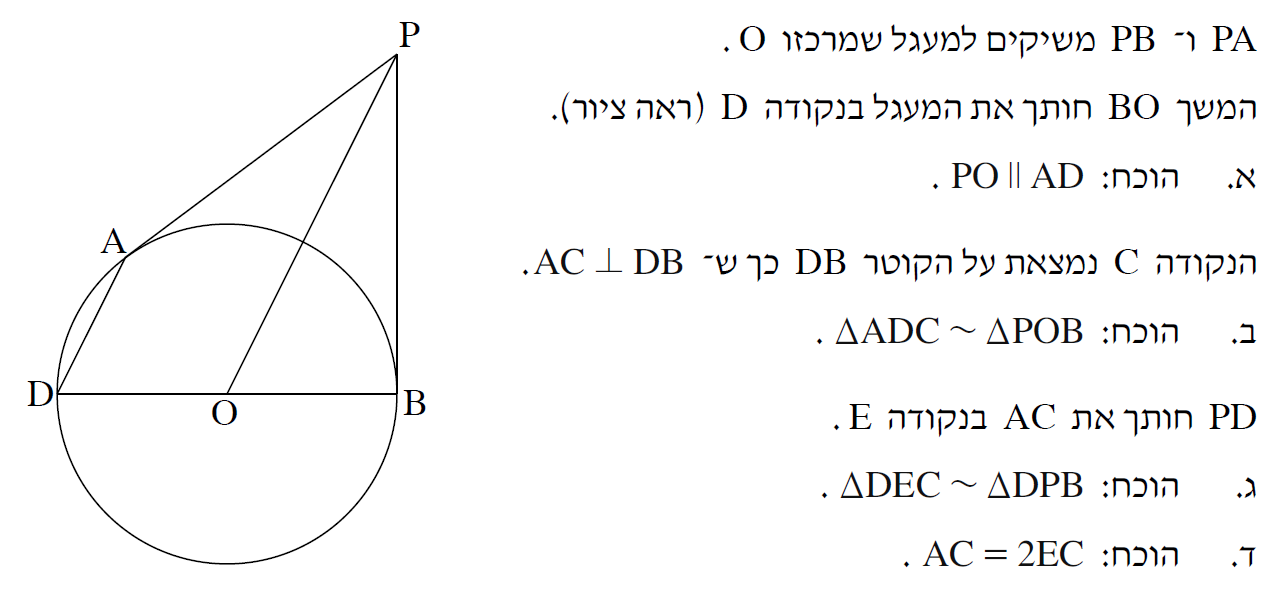
\includegraphics[width=\textwidth]{summer-2015a-4}
\end{center}

\textbf{סעיף א}
כאשר יש שני משיקים וקו מהנקודת החיתוך של המשיקים למרכז המעגל, עולה מיד שני משפטים: משפט
$(77)$
שהמשיקים האונכים לרדיוסים ומשפט
$(81)$
שהקו מנקודת החיתוך למרכז חוצה את הזווית. באיור, סימנו את חצאי הזווית ב-%
$\alpha$.
ניתן להשלים את שאר הזוויות )כאשר קיצרנו
$\beta = 90-\alpha$(
תוך שימוש בעובדות שסכום הזוויות במשולש וסכום הזוויות המשלימות לזווית שטוחה הם 
$180$.
בנוסף השתמשנו שוויון של רדיוסים כדי לקבל ש-%
$\triangle AOD$
הוא שווה שוקיים, ולכן
$\angle ADO=\angle DOA$.
כפי שניתן לראות,
$\angle ADO=\angle POB$
ולכן הן זוויות המאימות ו-%
$AD\perp PO$.

\begin{center}
\selectlanguage{english}
\begin{tikzpicture}[scale=1.2]
\coordinate [label=below:$O$] (O) at (0,0);
\coordinate [label=right:$B$] (B)  at (2.5,0);
\coordinate [label=above right:$P$] (P) at (2.5,4.5);
\node [draw,thick,circle through=(B),name path=circ] (circle) at (O) {};
\draw[thick,name path=tan1] (P) -- (B);
\path[name path=bd] (B) -- +(-5.2,0);
\path [name intersections={of=circ and bd,by={dummy,D}}];
\draw[thick] (B)--(O);
\draw[thick] (O) -- node[below] {$r$} (D);
\coordinate (A) at (tangent cs:node=circle,point={(P)},solution=1);
\draw[thick] (P) -- (A) -- (D);
\fill (O) node[above right,yshift=-2pt,xshift=2pt] {$\beta$} node[above,yshift=4pt,xshift=-1pt] {$\beta$} node[above left,yshift=-2pt,xshift=-4pt] {$2\alpha$} circle(1.5pt);
\fill (B) circle(1.5pt);
\fill (P) node[below left,yshift=-16pt,xshift=-14pt] {$\alpha$} node[below,yshift=-16pt,xshift=-5pt] {$\alpha$} circle(1.5pt);
\fill (D) node[left] {$D$} node[above right,yshift=-2pt,xshift=2pt] {$\beta$} circle(1.5pt);
\fill (A) node[above left] {$A$} node[below,yshift=-4pt] {$\beta$} circle(1.5pt);
\draw[thick] (P) -- (O);
\draw[thick,dashed] (O) -- node[above right,xshift=-2pt] {$r$} (A);
\draw[rotate=-60] (A) rectangle +(5pt,5pt);
\draw[rotate=90] (B) rectangle +(5pt,5pt);
\node at (-2.5,3.5) {$\beta = 90-\alpha$};
\end{tikzpicture}
\end{center}

\textbf{סעיף ב}

$AC\perp DB$
ו-%
$\angle ADC = \angle POB = \beta$,
ולכן
$\triangle ADC \sim \triangle POB$
לפי משפט
$(98)$
דמיון ז.ז.

\begin{center}
\selectlanguage{english}
\begin{tikzpicture}[scale=1.2]
\coordinate [label=below:$O$] (O) at (0,0);
\coordinate [label=right:$B$] (B)  at (2.5,0);
\coordinate [label=above right:$P$] (P) at (2.5,4.5);
\node [draw,thick,circle through=(B),name path=circ] (circle) at (O) {};
\draw[thick,name path=tan1] (P) -- (B);
\path[name path=bd] (B) -- +(-5.2,0);
\path [name intersections={of=circ and bd,by={dummy,D}}];
\draw[thick] (B)--(O);
\draw[thick] (O) -- (D);
\coordinate (A) at (tangent cs:node=circle,point={(P)},solution=1);
\draw[thick] (P) -- (A) -- (D);
\fill (O)  node[above right,yshift=-2pt,xshift=4pt] {$\beta$} circle(1.5pt);
\fill (B) circle(1.5pt);
\fill (P) node[below left,yshift=-16pt,xshift=-14pt] {$\alpha$} node[below,yshift=-16pt,xshift=-5pt] {$\alpha$} circle(1.5pt);
\fill (D) node[left] {$D$} node[above right,yshift=-2pt,xshift=14pt] {$\beta$} circle(1.5pt);
\fill (A) node[above left] {$A$} circle(1.5pt);
\draw[thick] (P) -- (O);
\draw[thick] (O) -- (A);
\draw[rotate=-60] (A) rectangle +(5pt,5pt);
\draw[rotate=90] (B) rectangle +(5pt,5pt);
\node at (-2.5,3.5) {$\beta = 90-\alpha$};
\draw[thick,dashed,name path=ac] (A) -- ($(D)!(A)!(B)$) node[below] {$C$} coordinate (C);
\draw[rotate=90] (C) rectangle +(5pt,5pt);
\draw[thick,dashed,name path=pd] (P) -- (D);
\draw[thick] (-2,0) arc[start angle=0,end angle=72,radius=4mm];
\path [name intersections={of=pd and ac,by={E}}];
\fill (E) node[right] {$E$} circle(1.5pt);=;
\end{tikzpicture}
\end{center}

\textbf{סעיף ג}
הזווית בנקדוה
$D$
משותפת ל-%
$\angle EDC$
ול-%
$\angle PDB$.
שני המשולשים הם ישר זווית ו-%
$\triangle DEC\sim \triangle DPB$
לפי דמיון ז.ז.

\textbf{סעיף ד}

מה יש לנו בצורה שערך אחד כפול לערך אחר. כמובן, שמדובר בקוטר ורדיוס. בסעיפים הקודמים הוכחנו ששני זוגות של משולשים דומים. נפשט את האיור ונראה אם אפשר למצוא את התשובה תוך שימוש במשולשים.
\begin{center}
\selectlanguage{english}
\begin{tikzpicture}[scale=1]
\coordinate [label=below:$O$] (O) at (0,0);
\coordinate [label=right:$B$] (B)  at (2.5,0);
\coordinate [label=above right:$P$] (P) at (2.5,4.5);
\node [circle through=(B),name path=circ] (circle) at (O) {};
\draw[thick,name path=tan1] (P) -- (B);
\path[name path=bd] (B) -- +(-5.2,0);
\path [name intersections={of=circ and bd,by={dummy,D}}];
\draw[thick] (B)-- node[below] {$r$} (O);
\draw[thick] (O) -- node[below,xshift=10pt] {$r$} (D);
\coordinate (A) at (tangent cs:node=circle,point={(P)},solution=1);
\draw[thick] (A) -- (D);
\fill (O) circle(1.5pt);
\fill (B) circle(1.5pt);
\fill (P) circle(1.5pt);
\fill (D) node[left] {$D$} circle(1.5pt);
\fill (A) node[above left] {$A$} circle(1.5pt);
\draw[thick] (P) -- (O);
\draw[rotate=90] (B) rectangle +(5pt,5pt);
\draw[thick,name path=ac] (A) -- ($(D)!(A)!(B)$) node[below] {$C$} coordinate (C);
\draw[rotate=90] (C) rectangle +(5pt,5pt);
\path [name intersections={of=pd and ac,by={E}}];
\fill (E) node[right,yshift=4pt] {$E$} circle(1.5pt);
\draw[thick] (E) -- (D) -- (P);
\end{tikzpicture}
\end{center}
\vspace{-25mm}
מסעיף ב
$\triangle ADC \sim \triangle POB$,
ולכן:
\[
\frac{AC}{PB} = \frac{DC}{OB} = \frac{DC}{r}\,.
\]
מסעיף ג
$\triangle DEC \sim \triangle DPB$,
ולכן:
\[
\frac{EC}{PB} = \frac{DC}{DB} = \frac{DC}{2r}\,.
\]
נצרף את שתי המשוואות:
\[
\frac{AC}{EC} = \frac{(PB\cdot DC)/r}{(PB\cdot DC)/2r}= 2\,.
\]


%%%%%%%%%%%%%%%%%%%%%%%%%%%%%%%%%%%%%%%%%%%%%%%%%%%%%%%%%%%%%%%%%%%

\section*{חורף תשע"ה}

\begin{center}
\selectlanguage{english}
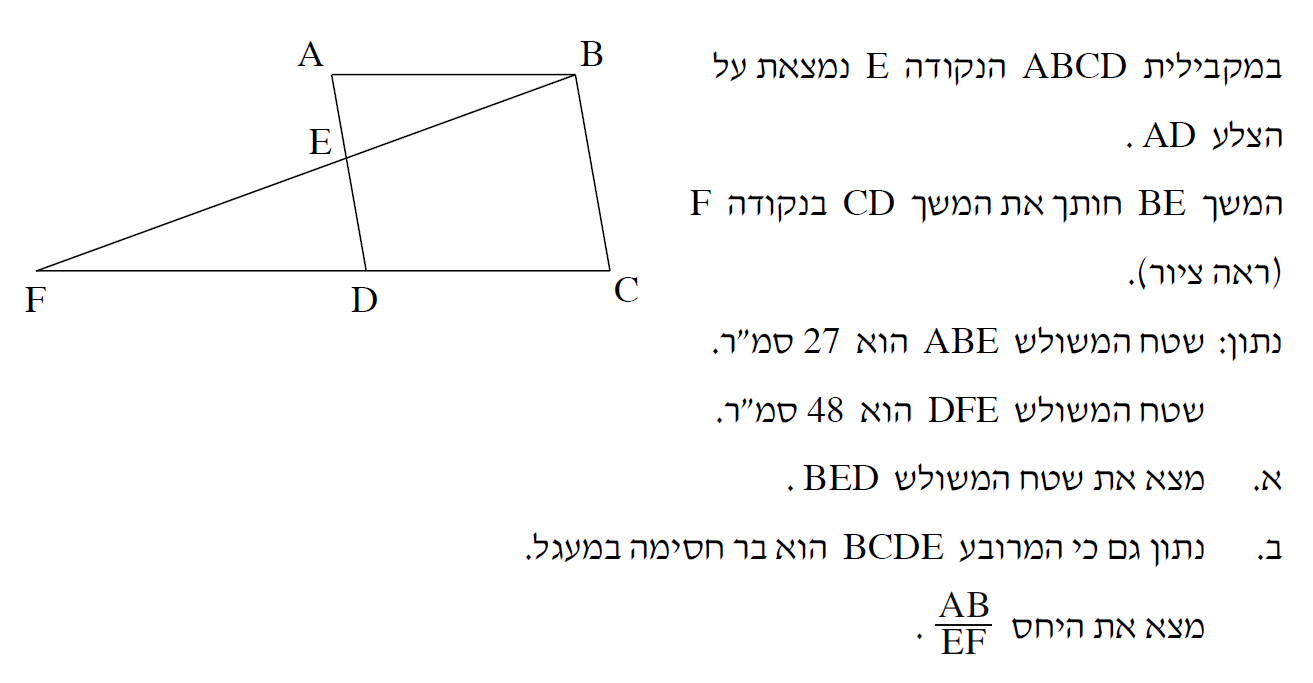
\includegraphics[width=\textwidth]{winter-2015-4}
\end{center}

\textbf{סעיף א}

\begin{center}
\selectlanguage{english}
\begin{tikzpicture}
\coordinate [label=below right:$D$] (D)  at (0,0);
\coordinate [label=below:$C$] (C)  at (4,0);
\coordinate [label=above right:$B$] (B)  at (3,3);
\coordinate [label=above left:$A$] (A)  at (-1,3);
\draw[thick,name path=para] (A) -- (B) -- (C) -- (D) -- cycle;
\node at (2,-.3) {$x$};
\node at (1.2,3.3) {$x$};
\path[name path=bf] (B) -- (-4,-.3);
\path[name path=df] (D) -- (-4,0);
\path[name intersections={of=bf and para,by={dummy,E}}];
\node[above left,xshift=-4pt] at (E) {$E$};
\path[name intersections={of=df and bf,by={F}}];
\node[below left] at (F) {$F$};
\draw[thick] (D) -- (F) -- (B);
\fill (A) circle (1.5pt);
\fill (B) circle (1.5pt);
\fill (C) circle (1.5pt);
\fill (D) circle (1.5pt);
\fill (E) circle (1.5pt);
\fill (F) circle (1.5pt);
\draw[thick,dashed] (E) |- (A);
\draw[thick,dashed] (E) |- (D);
\draw[thick,dashed] (B) -- (D);
\node at (-.1,2.4) {$h_1$};
\node at (-.8,.6) {$h_2$};
\end{tikzpicture}
\end{center}

ברור שהמשלושים
$\triangle ABE, \triangle DFE$
דומים בגלל הזוויות המתחלפות ב-%
$A,D$
ו-%
$B,F$.
לפי משפט
$100$
היחס בין הגבהים שווה לשורש היחס בין השטחים:
\[
\frac{h_1}{h_2} = \sqrt{\frac{S_{ABE}}{S_{DEF}}} = \sqrt{\frac{27}{48}} = \sqrt{\frac{9}{16}}=\frac{3}{4}\,.
\]
יש שתי שיטות לחשב את השטח של 
$\triangle BED$.
אפשר לראות שהשטח של המשולש שווה לnחצית שטח המקבילית פחות השטח של המשולש
$\triangle ABE$. 
)%
$DB$
הוא אלכסון ולכן השטח של המשולש
$\triangle ABD$
הוא מחצית שטח המקבילית.( סימנו את אורך הצלעות 
$AB, DC$
ב-%
$x$,
והשטח הוא:
\begin{eqnarray*}
S_{BDC} &=& \frac{1}{2}x(h_1+h_2) - \frac{1}{2}xh_1\\
&=& \frac{1}{2}x\left(h_1+\frac{4}{3}h_1-h_1\right)\\
&=& \frac{1}{2}x\cdot \frac{4}{3}h_1\\
&=& \frac{4}{3}\left(\frac{1}{2}xh_1\right)=\frac{4}{3}\left(S_{ABE}\right)= \frac{4}{3}\cdot 27 = 36\,.
\end{eqnarray*}

הדרך השנייה קשה לראות אבל החישוב מאוד פשוט. למשולשים 
$\triangle AEB,\triangle BED$
גובה זהה 
$h$
מהנקודה
$B$,
ולכן יחס השטחים הוא שורש יחס הצלעות
$AE,ED$
במשולשים 
$\triangle AEB,\triangle DFE$.
\begin{center}
\selectlanguage{english}
\begin{tikzpicture}
\coordinate [label=below right:$D$] (D)  at (0,0);
\coordinate (C)  at (4,0);
\coordinate [label=above right:$B$] (B)  at (3,3);
\coordinate [label=above left:$A$] (A)  at (-1,3);
\path[thick,name path=para] (A) -- (B) -- (C) -- (D) -- cycle;
\path[name path=bf] (B) -- (-4,-.3);
\path[name path=df] (D) -- (-4,0);
\path[name intersections={of=bf and para,by={dummy,E}}];
\node[above left,xshift=-4pt] at (E) {$E$};
\draw[thick] (A) -- (B) -- (E) -- cycle;
\draw[thick] (E) -- (D) -- (B);
\fill (A) circle (1.5pt);
\fill (B) circle (1.5pt);
\fill (D) circle (1.5pt);
\fill (E) circle (1.5pt);
\draw[thick,dashed] (B) -- node[above left] {$h$} ($(A)!(B)!(D)$);
\end{tikzpicture}
\end{center}
\vspace{-12mm}
\begin{eqnarray*}
\frac{S_{BED}}{S_{AEB}} &=& \frac{4}{3}\\
S_{BED} &=& \frac{4}{3}S_{AEB}=\frac{4}{3}\cdot 27 = 36\,.
\end{eqnarray*}

\vspace{-8mm}

\textbf{סעיף ב}

הנתון שהמרובע 
$BCDE$
בר חסימה במעגל מרמז למשפט
$(56)$
האומר שסכום הזוויות הנגדיות הוא 
$180^\circ$,
לכן קודם נסמן זוויות ואז נראה אם יוצא מזה משהו מועיל.
\begin{center}
\selectlanguage{english}
\begin{tikzpicture}[scale=1.1]
\coordinate [label=below right:$D$] (D)  at (0,0);
\coordinate [label=below:$C$] (C)  at (4,0);
\coordinate [label=above right:$B$] (B)  at (3,3);
\coordinate [label=above left:$A$] (A)  at (-1,3);
\draw[thick,name path=para] (A) -- (B) -- (C) -- (D) -- cycle;
\path[name path=bf] (B) -- (-4,-.3);
\path[name path=df] (D) -- (-4,0);
\path[name intersections={of=bf and para,by={dummy,E}}];
\node[above left,xshift=-4pt] at (E) {$E$};
\path[name intersections={of=df and bf,by={F}}];
\node[below left] at (F) {$F$};
\draw[thick] (D) -- (F) -- (B);
\fill (A) node[below right,xshift=2pt] {$\alpha$} circle (1.5pt);
\fill (B) node[below left,xshift=-22pt,yshift=1pt] {$\beta$} circle (1.5pt);
\fill (C) node[above left,xshift=-2pt] {$\alpha$} circle (1.5pt);
\fill (D) node[above left,xshift=-2pt] {$\alpha$} circle (1.5pt);
\fill (E) node[above,xshift=5pt,yshift=3pt] {$(\alpha)$} node[below,xshift=-5pt,yshift=-5pt] {$(\alpha)$} node[right,xshift=3pt,yshift=-5pt] {$(\alpha+\beta)$} circle (1.5pt);
\fill (F) circle (1.5pt);
\end{tikzpicture}
\end{center}
\vspace{-2mm}
הזוויות המוסמנות ב-%
$\alpha$
שוות בגלל זוויות מתחלפות ומתאימות במקבילית. נחשב את הזוויות המסומנות בסוגריים כך: 
$\angle AEB = 180 -(\alpha+\beta)$
כדי להשלים את זוויות המשולש ל-%
$180$,
ולכן הזווית המשלימה 
$\angle BED$
שווה ל-%
$180 - (180-(\alpha+\beta))=\alpha+\beta$\,.
לפי משפט
$(56)$:
\begin{eqnarray*}
\angle BCD + \angle BED &=& 180\\
\alpha + (\alpha + \beta) &=& 180\\
180-(\alpha+\beta) &=& \alpha\\
\angle AEB &=& \alpha\,,
\end{eqnarray*}
וגם 
$\angle FED=\alpha$
בגלל זוויות קודקודיות.

הפתעה נעימה: המשולשים
$\triangle AED, \triangle FED$ 
שווי שוקיים! זה מאפשר לנו להשתמש ביחס הנובע מהדמיון בין המשולשים שחישבנו בסעיף א.
$AB=EB$
ולכן
\[
\frac{AB}{EF} = \frac{EB}{EF} = \frac{3}{4}\,.
\]


%%%%%%%%%%%%%%%%%%%%%%%%%%%%%%%%%%%%%%%%%%%%%%%%%%%%%%%%%%%%%%%%%%%

\section*{קיץ תשע"ד מועד ב}

\begin{center}
\selectlanguage{english}
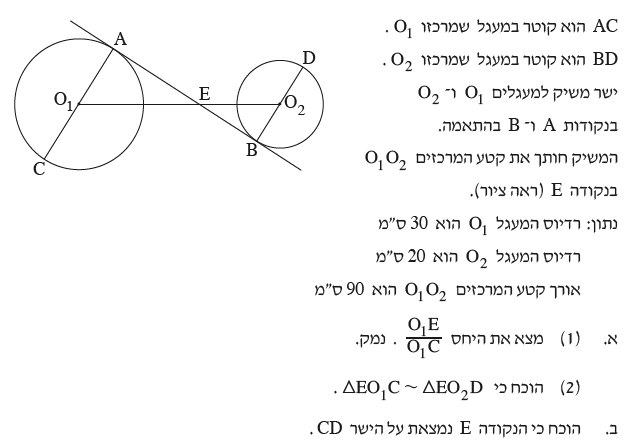
\includegraphics[width=\textwidth]{summer-2014b-4}
\end{center}

\vspace{-4ex}

\textbf{סעיף א}

\begin{center}
\selectlanguage{english}
\begin{tikzpicture}[scale=1.1]
\coordinate [label=left:$O_1$] (o1) at (0,0);
\coordinate [label=above:$A$] (A)  at (50:2);
\draw[rotate=-130] (A) rectangle +(4pt,4pt);
\coordinate [label=below:$C$] (C) at (-130:2);
\node [draw,circle through=(C)] at (o1) {};
\draw (A) -- (C);
\coordinate [label=right:$O_2$] (o2) at (5,0);
\coordinate [label=above:$D$] (D)  at ($(o2) + (50:1)$);
\coordinate [label=below:$B$] (B)  at ($(o2) + (-130:1)$);
\draw[rotate=50] (B) rectangle +(4pt,4pt);
\node [draw,circle through=(B)] at (o2) {};
\draw (B) -- (D);
\draw[name path=diameters] (o1) -- node[below,xshift=4mm] {\textsf{\small 90}} (o2);
\draw[name path=tangents] ($ (A) ! -.5 ! (B) $) -- ($ (A) ! 1.5 ! (B) $);
\path [name intersections={of=diameters and tangents,by={[label=above:$E$]E}}];
\path (A)  -- node[left] {\textsf{\small 30}} (o1);
\path (o1) -- node[left] {\textsf{\small 30}} (C);
\path (D)  -- node[right] {\textsf{\small 20}} (o2);
\path (o2) -- node[right] {\textsf{\small 20}} (B);
\path (o1) -- node[above] {$x$} (E);
%\draw[dashed] (C) -- (D);
\end{tikzpicture}
\end{center}

\medskip

$(1)$
משיק מאונך לרדיוס בנדוקת ההשקה שלו )משפט 77( ולכן המשולשים באיור הם ישר זווית. כדי לחשב את היחס
$\frac{O_1 E}{O_1 C}$
ננסה להוכיח שהמשולשים דומים.

הקו $AB$ משיק לשני המעגלים ולכן הזוויות
$\angle O_1 A E, \angle O_2 B E$
ישרות. הזוויות הקודקודיות
$\angle A E O_1, \angle B E O_2$
גם הן שוות. מכאן שהמשולשים
$\triangle O_1 A E, \triangle O_2 B E$
דומים )משפט 98, דמיון ז.ז.(. נסמן ב-%
$x$
את הקטע
$O_1 E$
ומהיחסים בין המשולשים הדומים נחשב את היחס המבוקש בשאלה:
\[
 \frac{O_1 E}{O_1 A}= \frac{x}{30} = \frac{O_2 E}{O_2B} = \frac{90-x}{20}\,, \quad\quad \frac{O_1 E}{O_1 C} = \frac{9}{5}\,.
\]

$(2)$
נראה שאפשר להשתמש באותה שיטה כדי להוכיח שהמשולשים 
$\triangle E O_1 C \sim \triangle E O_2 D$
דומים.
\begin{center}
\selectlanguage{english}
\begin{tikzpicture}[scale=1.1]
\coordinate [label=left:$O_1$] (o1) at (0,0);
\coordinate [label=above:$A$] (A)  at (50:2);
\draw[rotate=-130] (A) rectangle +(4pt,4pt);
\coordinate [label=below:$C$] (C) at (-130:2);
\node [draw,circle through=(C)] at (o1) {};
\draw (A) -- (o1);
\draw[dashed,very thick] (o1) -- (C);
\coordinate [label=right:$O_2$] (o2) at (5,0);
\coordinate [label=above:$D$] (D)  at ($(o2) + (50:1)$);
\coordinate [label=below:$B$] (B)  at ($(o2) + (-130:1)$);
\node[below right] at (o1) {$\theta$};
\node[above left,xshift=1mm] at (o2) {$\theta$};
\draw[rotate=50] (B) rectangle +(4pt,4pt);
\node [draw,circle through=(B)] at (o2) {};
\draw (B) -- (o2);
\draw[dashed,very thick] (o2) -- (D);
\draw[name path=diameters,dashed,very thick] (o1) -- node[below,xshift=6mm,yshift=-2mm] {\textsf{\small 90}} (o2);
\draw[name path=tangents] ($ (A) ! -.5 ! (B) $) -- ($ (A) ! 1.5 ! (B) $);
\path [name intersections={of=diameters and tangents,by={[label=above:$E$]E}}];
\path (A)  -- node[left,xshift=-1mm] {\textsf{\small 30}} (o1);
\path[dashed,very thick] (o1) -- node[left,xshift=-1mm] {\textsf{\small 30}} (C);
\path (D)  -- node[right,xshift=1mm] {\textsf{\small 20}} (o2);
\path (o2) -- node[right,xshift=1mm] {\textsf{\small 20}} (B);
\path[dashed,very thick] (o1) -- node[above] {$x$} (E);
\draw[dashed,very thick] (C) -- (D);
\end{tikzpicture}
\end{center}
אבל, כפי שמרמז סעיף ב, איננו יודעים שהנקודה
$E$
נמצאת על הקו הישר
$CD$,
ולכן איננו יכולים להניח ש-%
$\angle O_1 E C, \angle O_2 E D$
הן זוויות הקודקודיות )שוות(. במקום זה, נשתמש בעובדה שהקוטרים מקביליים ולהוכיח בצורה ישירה שהמשולשים דומים.

הקווים 
$AC,DB$
מקבילים אחד לשני כי שניהם ניצבים לאותו קו
$O_1,O_2$,
ולכן 
$\angle C O_1 E, \angle D O_2 E$
הן זוויות מתחלפות ושוות. כל הרדיוסים של מעגל שווים, כך ש-%
$O_1C=O_1A, O_2B=O_2D$.
מכאן שאפשר להשתמש בעובדה שהוכחנו ש-%
$\triangle E O_1 A \sim \triangle E O_2 B$
הם משולשים דומים כדי לראות שגם המשולשים
$\triangle E O_1 C \sim \triangle E O_2 D$
דומים.

\textbf{סעיף ב}
נתבונן בזוויות סביב הנקודה
$E$:
\begin{center}
\selectlanguage{english}
\begin{tikzpicture}[scale=1.1]
\coordinate [label=left:$O_1$] (o1) at (0,0);
\coordinate [label=above:$A$] (A)  at (50:2);
\coordinate [label=below:$C$] (C) at (-130:2);
\node [circle through=(C)] at (o1) {};
\draw (A) -- (C);
\coordinate [label=right:$O_2$] (o2) at (5,0);
\coordinate [label=above:$D$] (D)  at ($(o2) + (50:1)$);
\coordinate [label=below:$B$] (B)  at ($(o2) + (-130:1)$);
\node [circle through=(B)] at (o2) {};
\draw (B) -- (D);
\draw[name path=diameters] (o1) -- (o2);
\draw[name path=tangents] ($ (A) ! -.1 ! (B) $) -- ($ (A) ! 1.1 ! (B) $);
\path [name intersections={of=diameters and tangents,by={[label=above:$E$]E}}];
\path (A)  -- (o1);
\path (o1) -- (C);
\path (D)  -- (o2);
\path (o2) -- (B);
\path (o1) -- (E);
\node[xshift=-20pt,yshift=7pt] at (E) {$\alpha$};
\node[xshift=20pt,yshift=-7pt] at (E) {$\alpha$};
\node[xshift=38pt,yshift=6pt] at (E) {$\beta$};
\node[xshift=-38pt,yshift=-7pt] at (E) {$\beta$};
\draw (C) -- (D);
\end{tikzpicture}
\end{center}
הנקודה
$E$
נמצאת על 
$CD$
אם הזווית 
$\angle AED$
צמודה לזווית
$AEC$
)משפט 1(.


לאחר שהוכחנו את דמיון המשולשים
$\triangle O_1 E C\sim \triangle O_2 E D$
ו-%
$\triangle O_1 A E \sim \triangle O_2 B E$,
אפשר לסמן את הזוויות השוות
$\alpha$
ו-%
$\beta$.
נתון ש-%
$AB$
הוא קו ישר, ולכן 
$\angle AED$
צמודה ל-%
$\angle DEB$,
כך ש-%
$\angle AED = 180^\circ - \alpha - \beta$.
מכאן ש-%
$CD$
הוא קו ישר כי
$\angle CED = (180^\circ - \alpha - \beta) + \alpha + \beta = 180^\circ$.


\begin{center}
\textbf{\large העשרה: אין לסמוך על איורים!}
\end{center}
הנה הוכחה "נכונה"
\textbf{\R{שכל}}
משולש שווה שוקיים!

נתון משולש שרירותי 
$ABC$,
תהי
$P$
נקודת החיתוך בין חוצה הזווית של
$\angle A$
לבין האנך האמצעי של 
$BC$.
סמן ב-%
$E,F$
את נקודות החיתוך של האנחים מ-%
$P$
לצלעות
$AB,AC$.

המשולשים
$\triangle APE, \triangle APF$
חופפים כי הם משולשים ישר זווית עם זוויות שוות
$\alpha$
וצלע $AP$ משותף.
$BD=DC=a$
ולכן המשולשים
$\triangle DPB, \triangle DPC$
חופפים. מכאן ש-%
$PB=PC$
וגם המשלושים
$\triangle EPB, \triangle FPC$
חופפים ו-%
$AE+EB=AF+FC$,
$\triangle ABC$
שווה שוקיים.
\begin{center}
\selectlanguage{english}
\begin{tikzpicture}[scale=1]
\coordinate (P) at (0,0);
\node[xshift=4mm,yshift=1mm] at (P) {$P$};
\coordinate [label=left:$B$] (B)  at (-2,-2);
\coordinate [label=right:$C$] (C)  at (4,-2);
\coordinate [label=above:$A$] (A)  at (-1,2);
\node[below,yshift=-12pt,xshift=2pt] at (A) {$\alpha$};
\node[below,yshift=-12pt,xshift=15pt] at (A) {$\alpha$};
\draw (A) -- (B);
\draw (A) -- (C);
\draw (B) -- (C);
\draw (A) -- (P);
\draw (B) -- (P);
\draw (C) -- (P);
\coordinate[label=left:$E$] (E) at ($ (A) ! .44 ! (B) $);
\draw[rotate=-100] (E) rectangle +(4pt,4pt);
\draw (P) -- (E);
\coordinate[label=right:$F$] (F) at ($ (A) ! .33 ! (C) $);
\draw[rotate=-132] (F) rectangle +(4pt,4pt);
\draw (P) -- (F);
\coordinate[label=below:$D$] (D) at ($ (B) ! .33 ! (C) $);
\draw (D) rectangle +(4pt,4pt);
\draw (P) -- (D);
\node[left] at ($ (A) ! .5 ! (E) $) {};
\node[left] at ($ (B) ! .5 ! (E) $) {};
\node[below] at ($ (B) ! .5 ! (D) $) {$a$};
\node[below] at ($ (C) ! .5 ! (D) $) {$a$};
\node[right,xshift=2pt] at ($ (A) ! .5 ! (F) $) {};
\node[right,xshift=2pt] at ($ (C) ! .5 ! (F) $) {};
\end{tikzpicture}
\end{center}
הבעיה בהוכחה היא שהאיור אינו נכון כי הנקודה
$P$
נמצאות
\textbf{\R{מחוץ}}
למשולש:
\begin{center}
\selectlanguage{english}
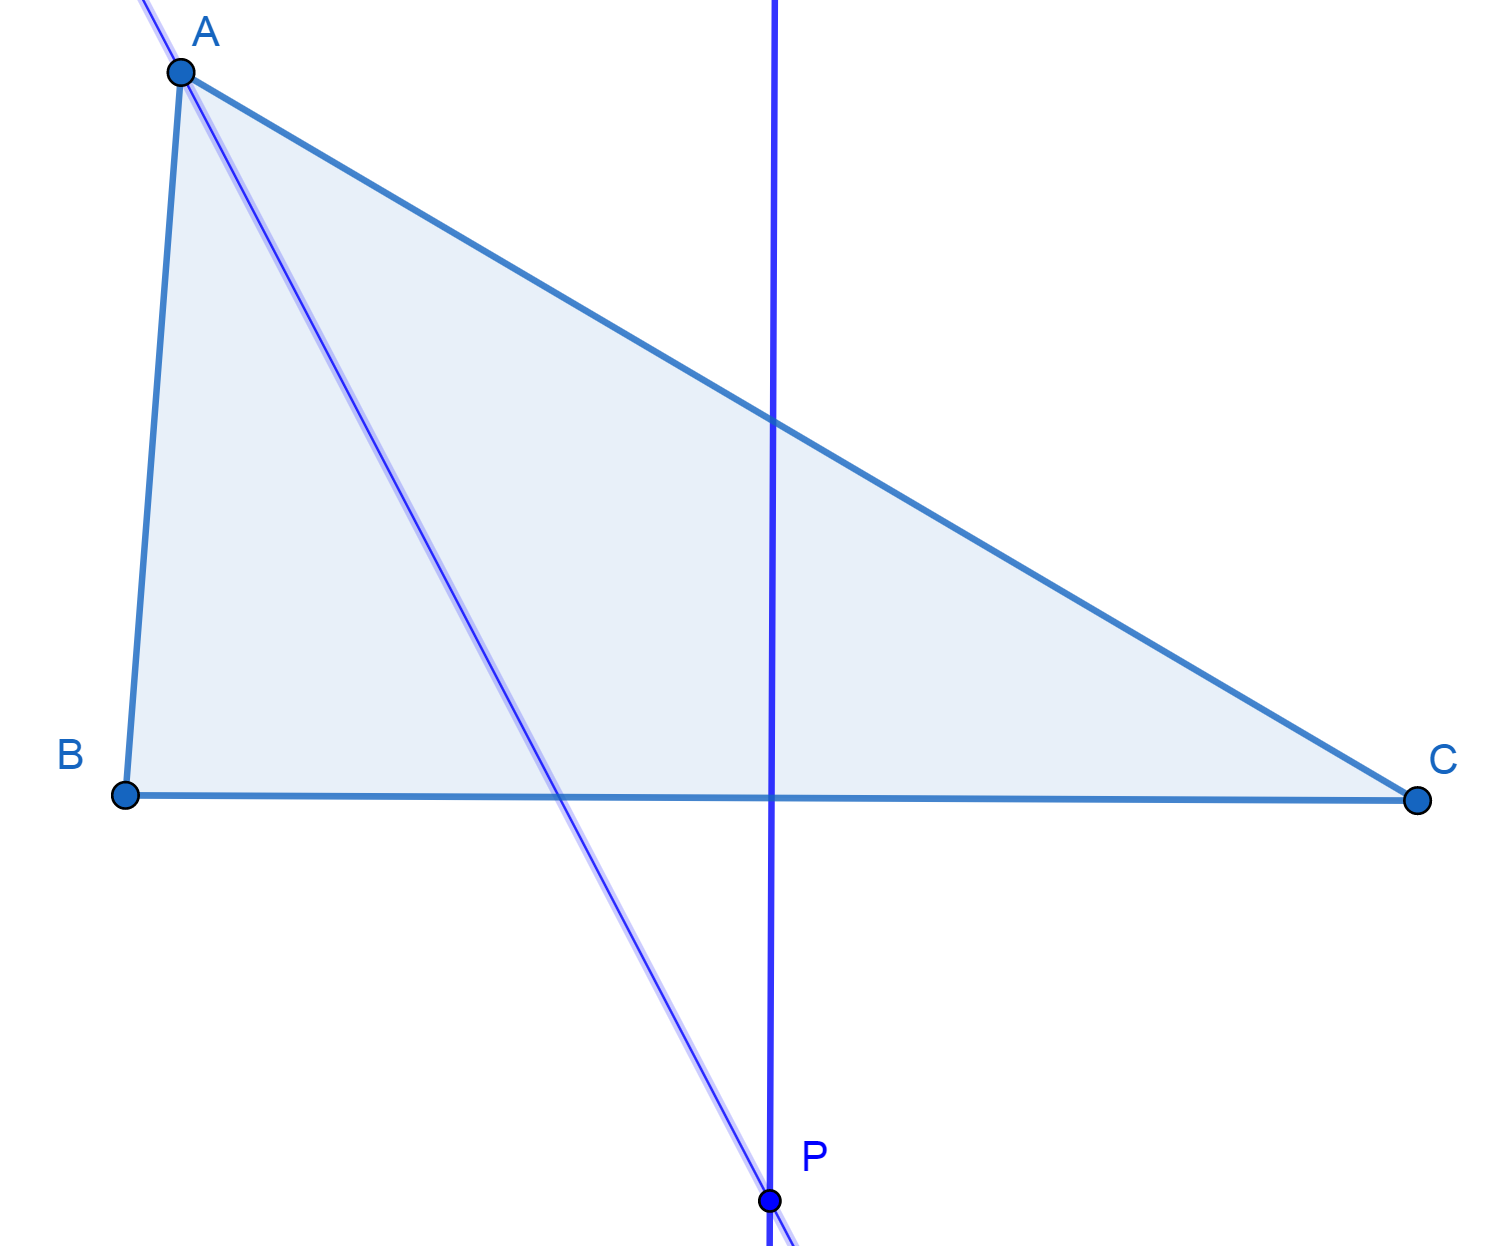
\includegraphics[width=.4\textwidth]{isoceles}
\end{center}


%%%%%%%%%%%%%%%%%%%%%%%%%%%%%%%%%%%%%%%%%%%%%%%%%%%%%%%%%%%%%%%%%%%
\section*{קיץ תשע"ד מועד א}

\begin{center}
\selectlanguage{english}
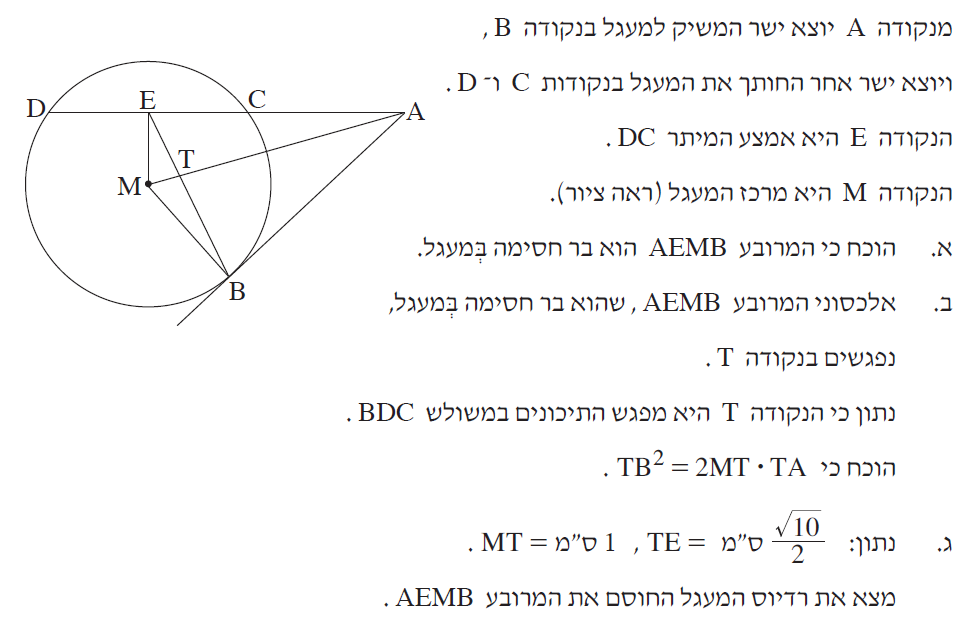
\includegraphics[width=\textwidth]{summer-2014a-4}
\end{center}


\textbf{סעיף א}
המשפטים שיכולים להיות שימושיים הם:
$(103)$
כאשר יש משיק וקו שחותך את המעגל, 
$AB^2=AC\cdot AD$.
$(77)$
הרדיוס והמשיק מאונכים זה לזה
$MB \perp PA$. 
$(68)$
קטע ממרכז המעגל החוצה מיתר מאונך למיתר.
$(56)$
ניתן לחסום מרובע במעגל רק אם סכום הזוויות הנגדיות שווה ל-%
$180^\circ$.

\begin{center}
\selectlanguage{english}
\begin{tikzpicture}[scale=1]
\coordinate [label=left:$M$] (M) at (0,0);
\coordinate [label=below right:$B$] (B)  at (-45:3);
\coordinate [label=right:$A$] (A) at (6,2);
\node [draw,thick,circle through=(B),name path=circ] at (M) {};
\draw[name path=tangents,thick] (A) -- ($ (A) ! 1.5 ! (B) $);
\path[name path=adc] (A) -- +(-9,0);
\path[name intersections={of=adc and circ,by={[label=above right:$C$]C,[label=above left:$D$]D}}];
\draw[thick] (A) -- (D);
\draw[thick,name path=am] (A) -- (M);
\draw[thick] (B) -- (M);
\path[name path=mid] (M) -- +(0,3.5);
\path[name intersections={of=mid and adc,by={[label=above:$E$]E}}];
\draw[thick,name path=eb] (E) -- (B);
\draw[thick] (E) -- (M);
\path[name intersections={of=eb and am,by={T}}];
\node[above,xshift=4pt] at (T) {$T$};
\fill (M) circle (1.5pt);
\fill (A) circle (1.5pt);
\fill (B) circle (1.5pt);
\fill (C) circle (1.5pt);
\fill (D) circle (1.5pt);
\fill (E) circle (1.5pt);
\end{tikzpicture}
\end{center}

משני המפשטים אנו יודעים ש-%
$\angle MEA + \angle MBA = 90^\circ + 90^\circ = 180^\circ$.
לפי משפט
$(106)$,
סכום הזוויות הפנימיות של מרובע הוא 
$360^\circ$,
ולכן:
\[
\angle EMB + \angle EAB = 360^\circ -(\angle MEA + \angle MBA) = 360^\circ - 180^\circ=180^\circ\,.
\]

\textbf{סעיף ב}

נכין איור עם המידע הרלוונטי בלבד. המעגל החוסם את המרובע
$AEMB$
והמשולש
$BDC$:
\vspace{-22mm}
\begin{center}
\selectlanguage{english}
\begin{tikzpicture}[scale=1]
\coordinate [label=left:$M$] (M) at (0,0);
\coordinate [label=below right:$B$] (B)  at (-45:3);
\coordinate [label=right:$A$] (A) at (6,2);
\node [circle through=(B),name path=circ] at (M) {};
\draw[name path=tangents,thick] (A) -- (B); %($ (A) ! 1.1 ! (B) $);
\path[name path=adc] (A) -- +(-9,0);
\path[name intersections={of=adc and circ,by={[label=above right:$C$]C,[label=above left:$D$]D}}];
\draw[thick,name path=am] (A) -- (M);
\draw[thick] (B) -- (M);
\path[name path=mid] (M) -- +(0,3.5);
\path[name intersections={of=mid and adc,by={[label=above left:$E$]E}}];
\draw[thick,name path=eb] (E) -- (B);
\draw[thick] (E) -- (M);
\path[name intersections={of=eb and am,by={T}}];
\node[above,xshift=4pt] at (T) {$T$};
\fill (M) circle (1.5pt);
\fill (A) circle (1.5pt);
\fill (B) circle (1.5pt);
\fill (C) circle (1.5pt);
\fill (D) circle (1.5pt);
\fill (E) circle (1.5pt);
\draw[thick,dashed] (C) -- (B) -- (D) -- cycle;
\tkzCircumCenter(M,E,A)\tkzGetPoint{O}
\tkzDrawCircle[thick](O,A)
\end{tikzpicture}
\end{center}
\vspace{-18mm}
אפשר לראות שקטעי הקווים
$MA,BE$
הם מיתרים נחתכים של המעגל החוסם. לפי משפט
$(101)$
$TB\cdot TE=MT\cdot TA$.
נתון שהנקודה
$T$
היא מפגש התיכונים, ולכן לפי משפט
$(46)$,
$TB/TE=2$.
כעת החישוב פשוט:
\begin{eqnarray*}
TB\cdot TE &=& MT\cdot AT\\
TB\cdot (TB/2) &=& MT\cdot AT\\
TB^2 &=& 2MT\cdot AT\,.
\end{eqnarray*}

\textbf{סעיף ג}
$\angle MBA$
היא זווית ישרה, ולכן לפי משפט
$(74)$
$MA$
הוא קוטר. עם הערכים הנתונים
$MT=1, TE=\frac{\sqrt{10}}{2}$
נחשב את הרדיוס:
\begin{eqnarray*}
R &=& \frac{1}{2}MA\\
&=&\frac{1}{2}(MT+TA)\\
%&=&\frac{1}{2}(1+TA)\\
&=&\frac{1}{2}(1+\frac{TB^2}{2\cdot 1})\\
&=&\frac{1}{2}(1+2TE^2)\\
&=&\frac{1}{2}(1+2\frac{10}{4})\\
&=&3\,.
\end{eqnarray*}

%%%%%%%%%%%%%%%%%%%%%%%%%%%%%%%%%%%%%%%%%%%%%%%%%%%%%%%%%%%%%%%%%%%


\section*{חורף תשע"ד}

\begin{center}
\selectlanguage{english}
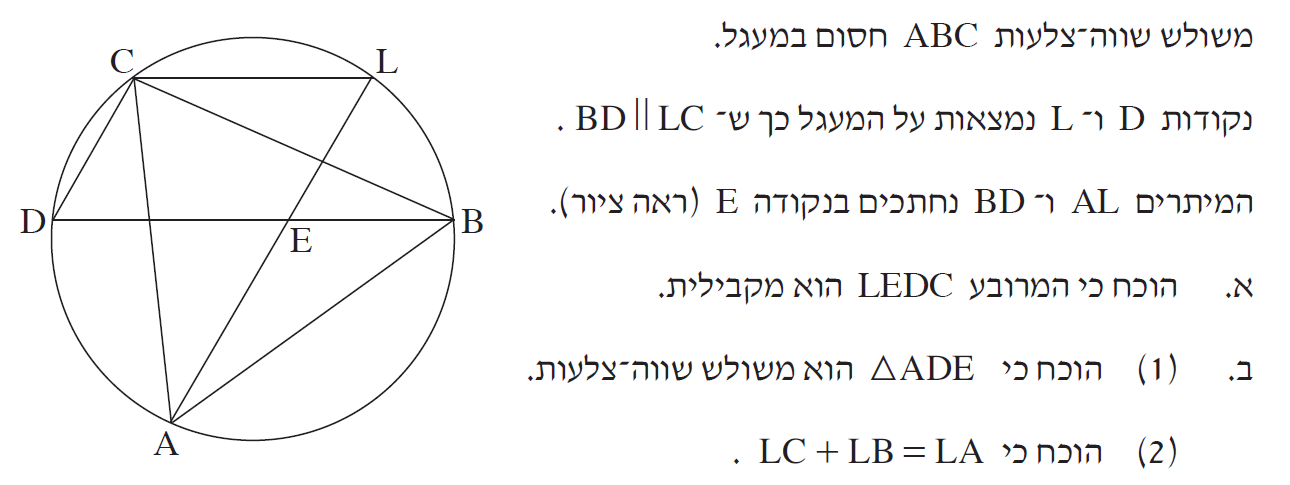
\includegraphics[width=\textwidth]{winter-2014-4}
\end{center}

\textbf{\R{סעיף א}}
אין לנו מידע על מיתרים המגדירים את המרובע שאמור להיות מקבילית, ולכן ננסה להוכיח אל ידי אפיון המקבילית כמרובע עם זוויות נגדיות שוות )משפט 92( או עם צלעות נגדיות מקביליות )משפט 03(. נתון שזוג אחד של צלעות
$CL,DE$
מקבילי, אז ננסה להוכיח שהזוג
$DC,EL$
מקבילי.

כאשר יש "מספר רב" של מיתרים, סביר שיש זוויות הנשענות על אותו מיתר או קשת ולכן הן שוות )משפטים 07,27(.

נסמן את הזוויות של המשלוש 
$\alpha=60^\circ$.
\begin{center}
\selectlanguage{english}
\begin{tikzpicture}%[scale=.75]
\coordinate (left) at (0,0);
\coordinate (right) at (6,0);
\coordinate (apath) at (0,-4);
\coordinate (bpath) at (7,1);
\coordinate (cpath) at (1.5,4);
\path [name path=chord1] (apath) -- (bpath);
\path [name path=chord2] (apath) -- (cpath);
\coordinate (center) at ($ (right)!.5!(left) $);
\node [draw,thick,circle through=(left),name path=circ] at (center) {};
\path [name intersections={of=circ and chord1,by={b,a}}];
\path [name intersections={of=circ and chord2,by={c,dummy1}}];
\fill (a) circle (2pt) node[below left] {$A$} node[xshift=4pt,yshift=15pt] {$\alpha$};
\fill (b) circle (2pt) node[right] {$B$} node[xshift=-15pt,yshift=-5pt] {$\alpha$};
\fill (c) circle (2pt) node[above left] {$C$} node[xshift=6pt,yshift=-10pt] {$\alpha$};
\path [name path=chord3] (b) -- +(-7,0);
\path [name intersections={of=circ and chord3,by={d}}];
\fill (d) circle (2pt) node[left] {$D$};
\path [name path=chord4] (c) -- +(4,0);
\path [name intersections={of=circ and chord4,by={l}}];
\fill (l) circle (2pt) node[above right] {$L$};
%% Draw triangle
\draw[thick] (a) -- (b) -- (c) -- cycle;
\draw[thick] (b) -- (d) -- (c) -- (l);
\draw[thick,name path=chord5] (l) -- (a);
\draw [name intersections={of=chord5 and chord3,by={e}}];
\fill (e) circle (2pt) node[below right] {$E$};
%% Angles
\draw[thick] +($ (a)!.15!(b) $) arc [radius=18pt,start angle=20,delta angle=82];
\draw[thick] ($ (c)!.15!(b) $) arc [radius=18pt,start angle=-20,delta angle=-75];
\draw[thick] ($ (b)!.15!(c) $) arc [radius=18pt,start angle=140,delta angle=82];
\end{tikzpicture}
\end{center}
$\angle CLA=\angle CBA$
כי הן נשענות על המיתר
$AC$.
$\angle CDB=\angle CAB$
כי הן נשענות על המיתר
$BC$.
נתון ש-%
$CL\|DB$
והזוויות המתחלפות שוות
$\angle LEB = \angle CLA$.
מכאן:
\begin{eqnarray*}
60^\circ=\angle CBA &=& \angle CLA =\angle LEB\\
60^\circ=\angle CAB &=& \angle CDB\,.
\end{eqnarray*}
$DC\|LE$
כי
$\angle LEB,\angle CDB$
הן זוויות מתאימות שוות.

\textbf{\R{סעיף ב}}
$(1)$
שוב, אין לנו מידע על אורכי הקווים לכן ננסה להוכיח שכל הזוויות של המשולש
$\triangle ADE$
שוות ל-%
$60^\circ$.
כמובן, שמספיק להוכיח ששתי זוויות שוות ל-%
$60^\circ$
כי השלישית צריכה להשלים ל-%
$180^\circ$,
סכום הזוויות במשולש.

בסעיף א הוכחנו ש-%
$\angle LEB=60^\circ$
ו-%
$\angle DEA=60^\circ$
כי הן זוויות קודקודיות. ננסה להוכיח ש-%
$\angle DAE=60^\circ$
או
$\angle ADE=60^\circ$
על ידי חיפוש זוויות אחרת הנשענת על אותו מיתר. בדיקה קצרה מראה ש-%
$\angle ACB=60^\circ, \angle ADE=\angle ADB$
נשענות על המיתר
$AB$.

$(2)$
נקח רמז מהחלק הראשון של הסעיף. אם
$\triangle ADE$
שווה צלעות, אז
$AE=DE$
ו-%
$DE=CL$
כי הן צלעות נגדיות של מקבילית. לכן:
\[
LA-LC=(LE+AE)-LC=(LE+LC)-LC=LE\,.
\]
נשאר להוכיח
$LE=LB$.
הוכחנו ש-%
$\angle LEB=60^\circ$,
כך שאם נוכיח שזווית נוספת ב-%
$\triangle LEB$
שווה ל-%
$60^\circ$
נקבל משלוש שווה צלעות ו-%
$LE=LB$.
שוב נחפש זוויות הנשענות על אותו מיתר ונקבל ש-%
$\angle BLA=\angle BCA$
כי שתיהן נשענות על המיתר
$AB$.

תוך כי נסיונות לפתור מצאתי הוכחה אחרת מעניינת. 
$\angle LBE=\angle LBD, \angle DCL$
נשענות או אותו קשה אבל
\textbf{מצדדים נגדיים}.
הזווית שנשענת על קשת שווה למחצית הקשת, ולכן אם סכום שתי הקשתות הוא כל המעגל, סכום הזוויות שווה 
$180^\circ$.
אנו יודעים ש-%
$\angle DCL=120^\circ$
כך ש-%
$\angle LBE=\angle LBD=60^\circ$.


\newpage

\section*{המלצות}

\begin{itemize}
\item
חשוב לצייר ציורים 
\textbf{וגדולים}.
בתהליך הפתרון אנו מסמנים את המידע המצטבר על הזוויות והצלעות ויש לדאוג שיהיה מספיק מקום.

\item
על הציורים להיות ברורים תוך שימוש בסרגל ומחוגה. אבל 
\textbf{אין לסמוך על הציור}.
לעתים, מה שנראה ברור בציור הוא בדיוק מה שעלינו להוכיח. בעמוד 
\L{\pageref{}}
הבאתי הוכחה שכל משולש הוא שווה שוקיים, כאשר ההוכחה מסתמכת על ציור שאינו נכון.

\item
לשאלות מספר סעיפים. במקרים רבים כדאי לצייר ציורים נפרדים לכל סעיף תוך העלמת מידע לא רלוונטי. בבחינה של בבבבב קל לראות את דרך הפתרון רק כאשר מסלקים קווים לא רלוונטיים.

\item
רצוי לרשום את המשפטים שיכולים להיות רלוונטיים לפני שמנסים לפתור את השאלה. זה יכול לכוון לפתרון. עם זאת יש לזכור שלא כל המשפטים נחוצים. בבחינה של בבבב היחס בין משיק לקו החותך מעגל נראה רלוונטי אבל אין בו צורך.

\item
יש משפטים שזוכרים בקלות כי הם די אינטואטיביים, למשל, שמשולשים חופפים לפי צ.צ.צ. ודומים לפי ז.ז. יש משפטים אחרים שקשה יותר לזכור אותם ושהוכחת נכונותם לא קלה. הכנתי מסמך: " " 
\url{}
עם ציוריים צבעוניים של מבחר משפטים כדי לעזור לזכור אותם. מה שקשה לזכור מניסוח מילולי מסורבל, קל לזכור מציור:
\begin{quote}
$45.$
שלושת התיכונים במשולש נחתכים בנקודה אחת.\\
$46.$
נקודת חיתוך התיכונים מחלקת כל תיכון ביחס 2:1.\\
)החלק הקרוב לקדקוד הוא פי 2 מהחלק האחר(.
\end{quote}
\begin{center}
\selectlanguage{english}
\begin{tikzpicture}[scale=1.1]
\coordinate (a) at (0,0);   % Points of the triangle
\coordinate (b) at (6,0);
\coordinate (c) at (4,3);
% Coordinates of bisectors
\coordinate (ab) at ($(a)!.5!(b)$);
\coordinate (bc) at ($(b)!.5!(c)$);
\coordinate (ac) at ($(a)!.5!(c)$);
% Draw the triangle and bisectors
\draw[blue,very thick] (a) -- node[above] {$\bm{x}$} (ac) -- node[above] {$\bm{x}$} (c);
\draw[red,very thick] (b) -- node[right] {$\bm{y}$} (bc) -- node[right] {$\bm{y}$} (c);
\draw[green!60!black,very thick] (a) -- node[below] {$\bm{z}$} (ab) -- node[below] {$\bm{z}$} (b);
\draw[very thick,red,name path=da] (a) -- (bc);
\draw[very thick,blue,name path=db] (b) -- (ac);
\draw[very thick,green!60!black,name path=dc] (c) -- (ab);
% Get their intersection
\path [name intersections={of=da and db,by={intersection}}];
% Labels
\path (a) -- node[above,red] {$\bm{2a}$} (intersection);
\path (bc) -- node[above,red] {$\bm{a}$} (intersection);
\path (b) -- node[above,blue] {$\bm{2b}$} (intersection);
\path (ac) -- node[above,blue] {$\bm{b}$} (intersection);
\path (c) -- node[right,green!60!black] {$\bm{2c}$} (intersection);
\path (ab) -- node[right,green!60!black] {$\bm{c}$} (intersection);
% Points at the intersections
\fill (intersection) circle (2pt);
\fill (ab) circle (2pt);
\fill (ac) circle (2pt);
\fill (bc) circle (2pt);
\end{tikzpicture}
\end{center}

\end{itemize}

%\end{comment}

\end{document}
